The guidance system divides into two parts: a waypoint generator and a lookahead-based guidance law. The objective of the waypoint generator is to the lookahead-based guidance of the local goals (i.e., waypoints), while the look ahead guidance guides the spaceship toward such goals (in this case, we use desired velocity as our guidance output).

\subsubsection{Waypoint Generator}
The waypoint generator encoded the spaceship's airspace defense mission, as shown in Table~\ref{tab:waypoint} and Fig.~\ref{fig:exp_Dgain}. 

\begin{table}[!h]
	\caption{Airspace defense mission and the corresponding waypoints}
	\centering
	
	\begin{tabular}{@{}cll@{}}
		\toprule
		\textbf{\rotatebox[origin=c]{0}{ {index}}}  & 
		\textbf{\rotatebox[origin=c]{0}{waypoint (km)}}& 
		\textbf{\rotatebox[origin=c]{0}{description}}
		\\ \toprule
		1 & (x,y,z) = (0,0,0) & start location\\ 
		2 & (x,y,z) = (0,0,1) & vertical take off\\ 
		3 & (x,y,z) = (10,0,5) & departure \\ 
		4 & (x,y,z) = (30,30,100) & climb\\ 
		5 & (x,y,z) = (10,20,5) & descent \\ 
		6 & (x,y,z) = (7,7,5) & initial approach\\ 
		7 & (x,y,z) = (4,4,3) & middle approach\\ 
		8 & (x,y,z) = (0,0,3) & final approach \\ 
		10 & (x,y,z) = (0,0,0) & vertical landing \\ 
		\bottomrule
	\end{tabular}
	\label{tab:waypoint}
\end{table}

The objective of the mission is to navigate between those waypoints in straight lines. To deal with noise and disturbance, the waypoint generator output new waypoints only if the spaceship reaches the acceptance sphere, i.e., equation~\ref{eq:acceptance_sphere} is satisfied.
\begin{equation}
	||p^w(t) - p_i^{w*} || \leq \epsilon_r,
	\label{eq:acceptance_sphere}
\end{equation}
where $p^w(t)$ denotes the position of the x-wing fighter with respect to world-fixed frame, $p_i^{w*}$ denotes the $i^th$ waypoint, $||\square||$ denotes the second norm, and $\epsilon_r$ denotes the radius of the acceptance sphere which is set to a relatively small value of 2 km to ensure following the desired path. 


\subsubsection{Lookahead-based Guidance Law}
To follow the path described previously, lookahead-based line-of-sight guidance law is implemented. This approach includes two objectives: guiding the spaceship (1) toward and (2) to follow the path segment, i.e., straight line segment connecting between the previous and next waypoints.

\begin{figure}[h]
		\centering
		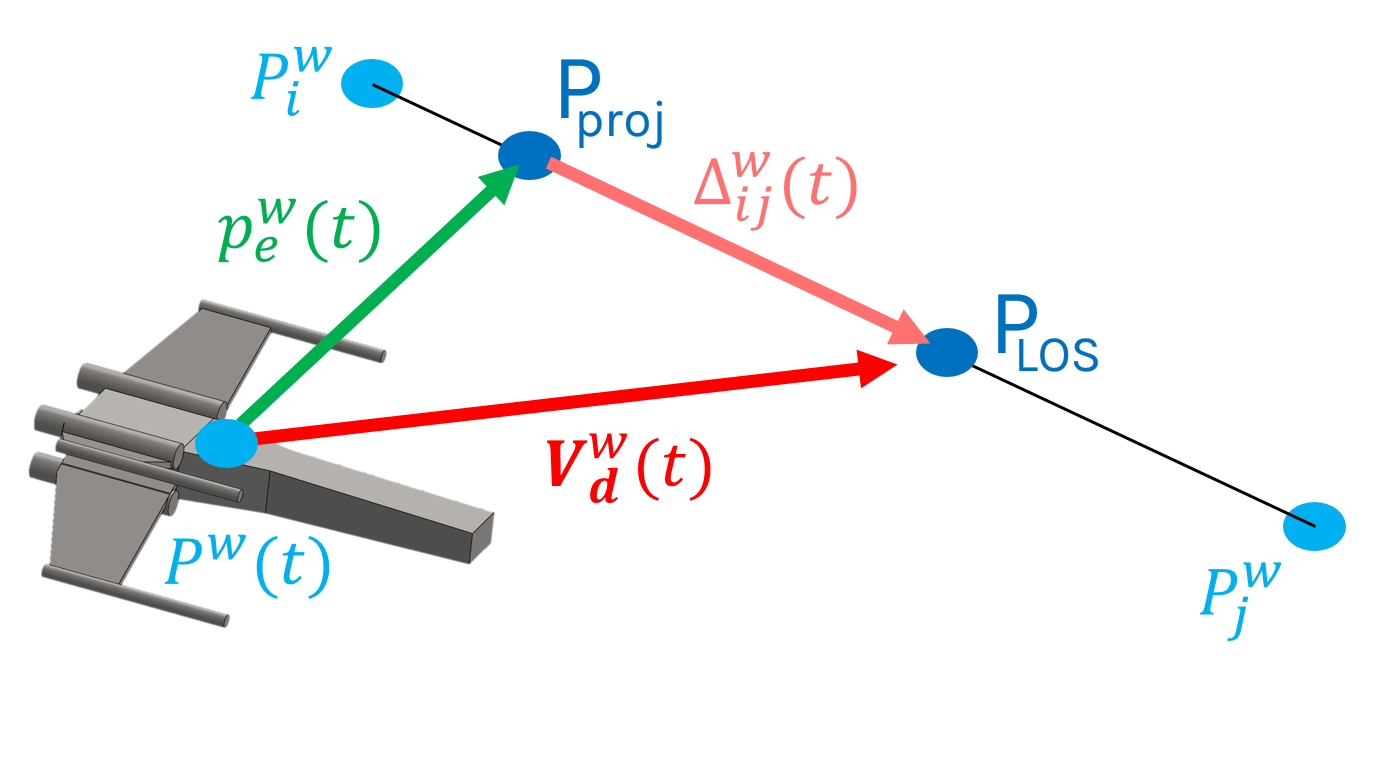
\includegraphics[width=0.7\linewidth]{figures/lookahead_normal.png}
	\caption{Graphic representation of line-of-sight position and the guidance/desired velocity.}
	\label{fig:lookahead}
\end{figure}

The line-of-sight position is computed according to:
\begin{equation}
p^w_{los}(t) = p^w_i + \Delta^w_{ij}(t) + p^w_e(t),
\label{eq:guidance_plos}
\end{equation}
where $p^w_{los}(t)$ denotes the light-of-sight position at time $t$, $p^w_i$ denotes the previous waypoint, $\Delta^w_{ij}(t)$ denotes the lookahead distance, and $p^w_e(t)$ denotes the distance toward the path segment. Note that, here, all value is computed with respect to the world-fixed frame.

The lookahead distance ($\Delta^w_{ij}(t)$) guides the spaceship to follow the path. It is computed from the unit vector of path segment according to:
\begin{equation}
\Delta^w_{ij}(t) = \frac{  \eta_\Delta  (p_j^i)}{||p_j^i||+\epsilon},
\label{eq:guidance_delta}
\end{equation}
where $p_j^i$ denotes the vector from the previous waypoint to the next waypoint, or rather, $p_j^i = p^w_j-p^w_i$, $\eta_\Delta$ denotes the gain defining the magnitude of lookahead distance (this parameter is analyzed in section~\ref{sec:exp_guidance}), and $\epsilon$ denotes an arbitrary small number which is $1.0\times10^{-6}$ in this case.

On the other hand, the distance toward the path ($p^w_e(t)$) guides the spaceship toward the path. It is computed from the projection point ($P_{proj}$) according to:
\begin{equation}
p^w_e(t) = \eta_e \left(    \frac{          (  p^i(t) \cdot p_j^i  )    p_j^i        }{||p_j^i||^2+\epsilon}         -p^i(t)  \right),
\label{eq:guidance_pe}
\end{equation}
where $p^i(t)$ denotes the vector from the previous waypoint to the spaceship's position, or rather, $p^i(t) = p^w(t)-p^w_i$, and $\eta_e$ denotes the gain defining the magnitude of lookahead distance (this parameter is analyzed in section~\ref{sec:exp_guidance}).

Lastly, the guidance/desired velocity ($v_d^w(t)$) is computed from:
\begin{equation}
v^w_d(t) = \left( p^w_{los}(t)-p^w(t) \right).
\label{eq:guidance_velocity}
\end{equation}


